%%%%%%%%%%%%%%%%%%%%%%%%%%%%%%%%%%%%%%%%%
% University/School Laboratory Report
% LaTeX Template
% Version 3.1 (25/3/14)
%
% This template has been downloaded from:
% http://www.LaTeXTemplates.com
%
% Original author:
% Linux and Unix Users Group at Virginia Tech Wiki 
% (https://vtluug.org/wiki/Example_LaTeX_chem_lab_report)
%
% License:
% CC BY-NC-SA 3.0 (http://creativecommons.org/licenses/by-nc-sa/3.0/)
%
%%%%%%%%%%%%%%%%%%%%%%%%%%%%%%%%%%%%%%%%%

%----------------------------------------------------------------------------------------
%	PACKAGES AND DOCUMENT CONFIGURATIONS
%----------------------------------------------------------------------------------------

\documentclass{article}

\usepackage[version=3]{mhchem} % Package for chemical equation typesetting
\usepackage{siunitx} % Provides the \SI{}{} and \si{} command for typesetting SI units
\usepackage{graphicx} % Required for the inclusion of images
\usepackage{natbib} % Required to change bibliography style to APA
\usepackage{amssymb,amsmath,amsthm}
\usepackage{booktabs}

\setlength\parindent{0pt} % Removes all indentation from paragraphs

\renewcommand{\labelenumi}{\alph{enumi}.} % Make numbering in the enumerate environment by letter rather than number (e.g. section 6)

%\usepackage{times} % Uncomment to use the Times New Roman font

%----------------------------------------------------------------------------------------
%	DOCUMENT INFORMATION
%----------------------------------------------------------------------------------------

\title{Solving the Wave Equation\\On a Curvilinear Grid Using MPI\\ CS/MATH 471} % Title

\author{Teo Brandt and Brennan Collins} % Author name

\date{\today} % Date for the report

\begin{document}

\maketitle % Insert the title, author and date



% If you wish to include an abstract, uncomment the lines below
\begin{abstract}
\begin{figure}[h]
\centering
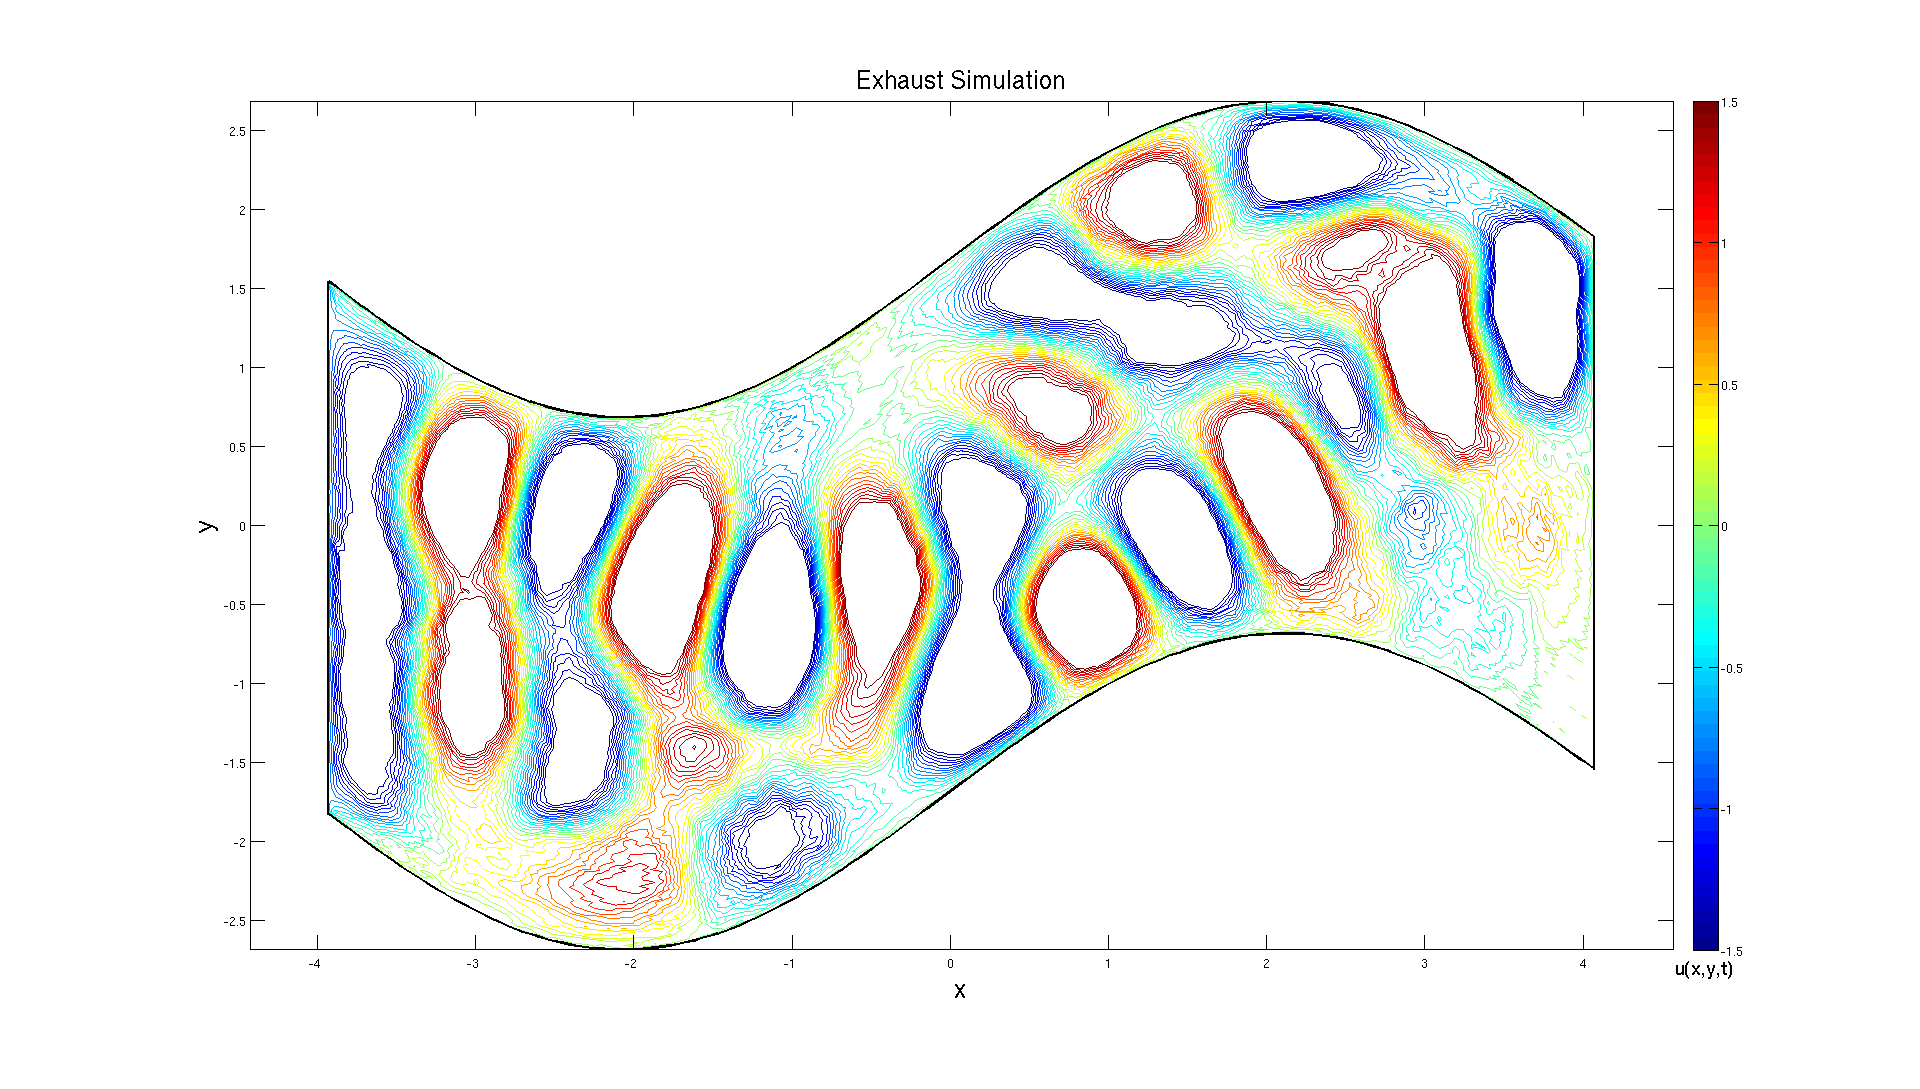
\includegraphics[width=1.0\textwidth]{exhaust_sim_10}
\end{figure}
In this report the hyperbolic equation known as the 2D wave equation is presented with a constant coefficient
\[
u_{tt}=c(u_{xx}+u_{yy})+F(x,y,t),\text{   }(x,y)\in \Omega, t\>0,
\]
with Dirichlet boundary conditions
\[
u(x,y,t)=g(x,y,t),\text{   }\forall (x,y) \in \delta \Omega,
\]
and initial conditions
\[
u(x,y,0) = f(x,y),\text{   }u_{t}(x,y,0)=h(x,y), \forall (x,y) \in \Omega
\]
\end{abstract}
\newpage
%----------------------------------------------------------------------------------------
%	SECTION 1
%----------------------------------------------------------------------------------------

\section{Objective}

In this project we will restrict the geometry \(\Omega\) to be a logically square shaped domain, assuming that there is a smooth mapping \((x,y)=(x(r,s),y(r,s))\) from the reference element \(\Omega_{R}=\big\{(r,s)\in[\-1,1]\ ^{2}\) to \(\Omega\).
\\
The domains that will be considered in this report are shown below.
\begin{figure}[htp]

\centering
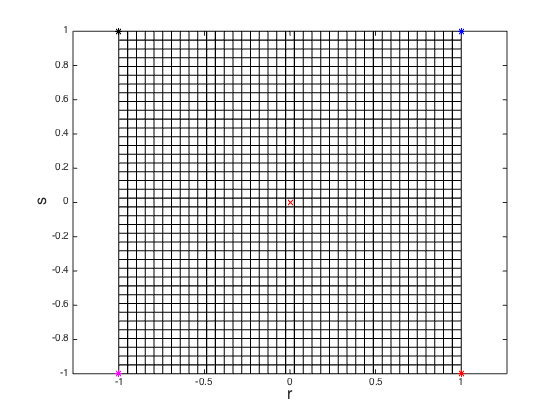
\includegraphics[width=.3\textwidth]{squaremap}\hfill
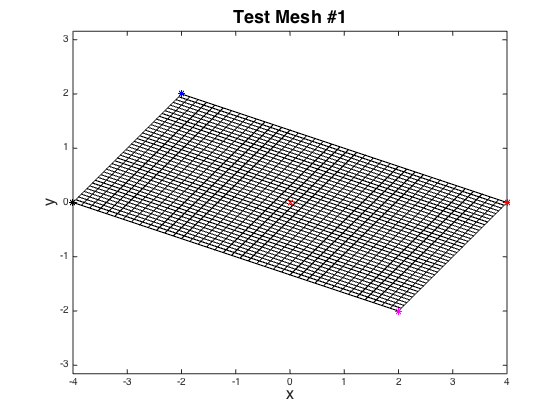
\includegraphics[width=.3\textwidth]{rectmap}\hfill
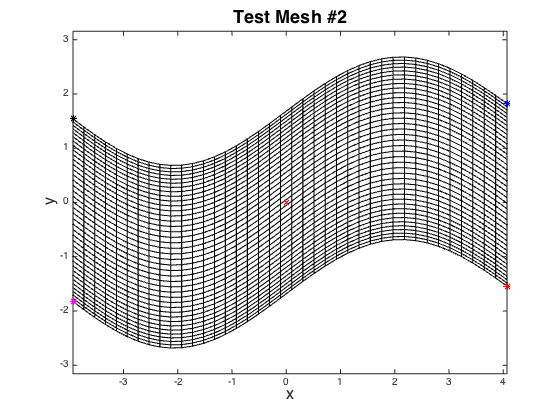
\includegraphics[width=.3\textwidth]{exhaustmesh}

\caption{Spacial Domains 1-3}
\label{fig:figure3}

\end{figure}

% If you have more than one objective, uncomment the below:
%\begin{description}
%\item[First Objective] \hfill \\
%Objective 1 text
%\item[Second Objective] \hfill \\
%Objective 2 text
%\end{description}

\subsection{Details}
In the \((r,s)\) coordinate system the wave equation takes the form: \cite{hw}
\[
Ju_{tt}=c\bbig((Jr_{x}(r_{x}u_{r}+s_{x}u_{s})+Jr_{y}(r_{y}u_{r}+s_{y}u_{s}))_{r}
\]
\[
+ (Js_{x}(r_{x}u_{r}+s_{x}u_{s})+Js_{y}(r_{y}u_{r}+s_{y}u_{s}))_{s}\bbig)
\]
\[
+JF(x,y,t),\text{   }(x,y)\in \Omega, t\>0
\]
where the metrics and jacobian are
\[
s_{x}=\frac{-y_{r}}{x_{r}y_{s}-x_{s}y_{r}}; s_{y}=\frac{x_{r}}{x_{r}y_{s}-x_{s}y_{r}}; r_{x}=\frac{y_{s}}{x_{r}y_{s}-x_{s}y_{r}}; r_{y}=\frac{-x_{s}}{x_{r}y_{s}-x_{s}y_{r}}
\]
and
\[
J(r,s)=x_{r}y_{s}-x_{s}y_{r}
\]
respectively.
\\
 
%----------------------------------------------------------------------------------------
%	SECTION 2
%----------------------------------------------------------------------------------------

\section{Parallelization Assignments}

The first step in parallelizing the problem is to decompose the domain in a way that minimizes communication between processors. The best choice in this case is to take a 2-dimensional decomposition. The decomposition that works best here for an \(MxN\) domain with P processors is to break the domain into \(P = X_{m} * Y_{m}\) sections, where
\(\bigg|\frac{M}{X_{m}} - \frac{N}{Y_{m}}\bigg|\) is minimized. 

Once \(\bigg|\frac{M}{X_{m}} - \frac{N}{Y_{m}}\bigg|\) is minimized, we find \(px\) and \(py\) for each processor. Each processor is assigned an ID, which is a value from 0 to P-1. Using this ID along with the \(X_{m}\) and \(Y_{m}\) found above, we can assign \(px\) and \(py\) as follows:
\[
px = \frac{ID}{X_{m}} + 1
\]
\[
py = ID mod Y_{m} + 1
\]

This assigns a unique (px,py) pair to each processor. We can also use the ID to determine our neighbors. Our north neighbor then would simply be ID - 1, the south neighbor would be ID + 1, the west neighbor will be \(ID - Y_{m}\), and the east neighbor will be \(ID + Y_{m}\).

Now that neighbors are assigned, we can perform communication effectively, similar to how it was done in the 1-D domain decomposition. The main difference is that communication is not just between left and right neighbors, but also top and bottom.

To ensure that communication was proceeding as expected, a test was added where each node sent its ID to its direct neighbors (N,S,E,W) and then write the updated to a file. Upon inspection of the file, the edges of array corresponded to IDs of the node's immediate neighbors, so 2-D communication is properly implemented.

%----------------------------------------------------------------------------------------
%	SECTION 3
%----------------------------------------------------------------------------------------
\section{Discretization in Time and Space}

For discretization in time, we use a simple centered difference formula
\[
u_{tt}(x_{i},y_{j},t_{n})\approx \frac{v_{i,j}^{n+1}-2v_{i,j}^{n}+v_{i,j}^{n-1}}{(\Delta t)^{2}}
\]
One of the problems that occurred in the discretization of time for each processor, is that each node has its own matrices independent of the other processors. Since this is the case, each node will have its own unique Jacobian. Previously, the timestep in each processor was set right before the discretization loop, each processor was using its own Jacobian to set this timestep. Since the Jacobian could be unique for each node, then the size of the timestep and transitively the number of timesteps in the discretization loop for time could be different from processor to processor. That means that some of the processors will get through this loop before others. The processors that re-enter the loop will go on to make a \textit{mpi\_sendrecv} call to a neighbor that has completely passed through the loop, meaning that the call will go unanswered, and the node will enter deadlock. The solution was simple, to remove the Jacobian from the setting of the timestep and replace it with a numerical constant.

%----------------------------------------------------------------------------------------
%	SECTION 4
%----------------------------------------------------------------------------------------

\section{Manufactured Solution}

The manufactured solution is tool that allows the algorithm to be tested against a known solution \(v\) to the numerical approximation \(u\) that we wish to achieve. In this case
\[
u_{tt}=c(u_{xx}+u_{yy})+F(x,y,t),\text{   }(x,y)\in \Omega, t\>0,
\]
\[
u(x,y,t)=g(x,y,t),\text{   }\forall (x,y) \in \delta \Omega,
\]
\[
u(x,y,0) = f(x,y),\text{   }u_{t}(x,y,0)=h(x,y), \forall (x,y) \in \Omega
\]

By measuring error
\[
\epsilon_{p}(t)=\Big(\integral_{0}^{1}\bigg|u-v\bigg|^{p}dx\Big)^{\frac{1}{p}}
\]
for some different values of \(h\) we can verify that order of our approximation is \(\epsilon_{p}\sim O(h^{r})\) as we expect. The results of testing the trigonometric manufactures solution of the form
\[
u(x,y,t)=sin(t-x)*sin(y)
\]
for the domains referenced in fig.1 are given
\begin{figure}[h]
\caption{MMS convergence}
\centering
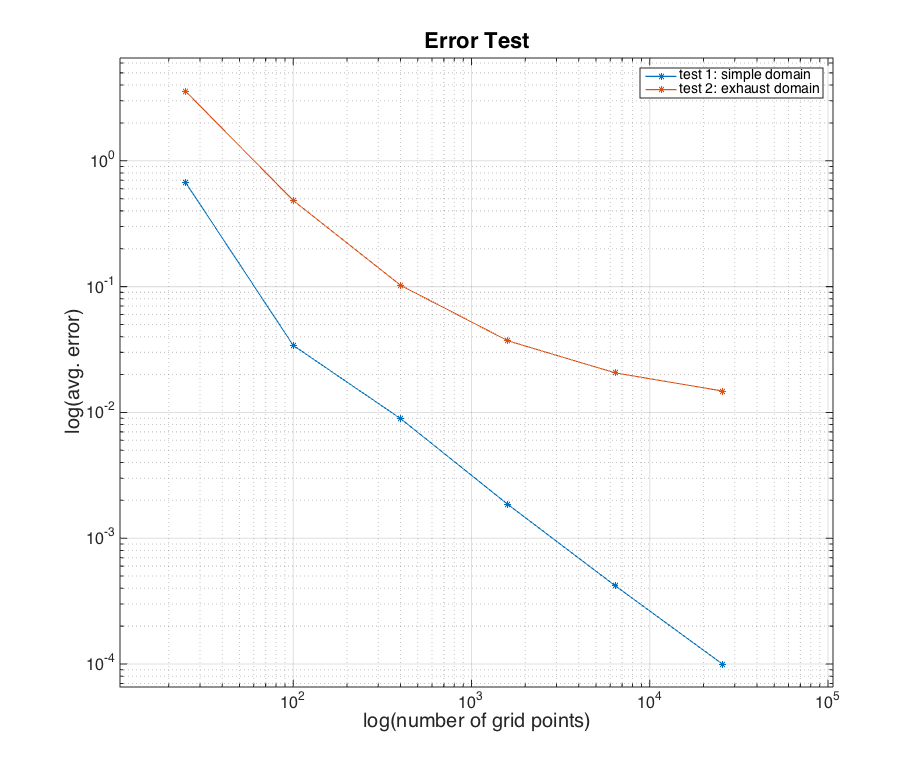
\includegraphics[width=0.5\textwidth]{ErrorTest_TrigMMS}
\end{figure}
In the figure it is important to note that the error is plotted against the number of grid points, which in this experiment was square \(nx=ny\) so the order 1 shown is actually order 2.
%----------------------------------------------------------------------------------------
%	SECTION 5
%----------------------------------------------------------------------------------------

\section{The Simulation of the Exhaust}

The theory up to this point has been in preparation for a discussion and presentation of our approximation of the complicated curvilinear coordinate system shown below again for convenience
\begin{figure}[h]
\caption{Exhaust Grid}
\centering
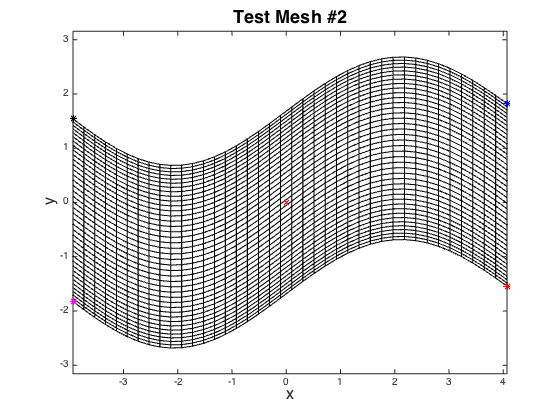
\includegraphics[width=0.5\textwidth]{exhaustmesh}
\end{figure}
with the smooth mapping
\[
x(r,s) = 4r+2sin(r)*0.05sin(r)
\]
\[
y(r,s) = sin(3r)+2sin(s)
\]
For this system boundary conditions were set as follows
\[
u(0,y,0) = 2sin(5t)
\]
\[
u(right,y,0) = 0
\]
\[
u(x,bottom,0) = 0
\]
\[
u(x,top,0) = 0
 \]
 
The simulation was run for 10 "seconds" or \(\sim700 timesteps\).
\begin{figure}[h]
\caption{Exhaust Simulation Results}
\centering
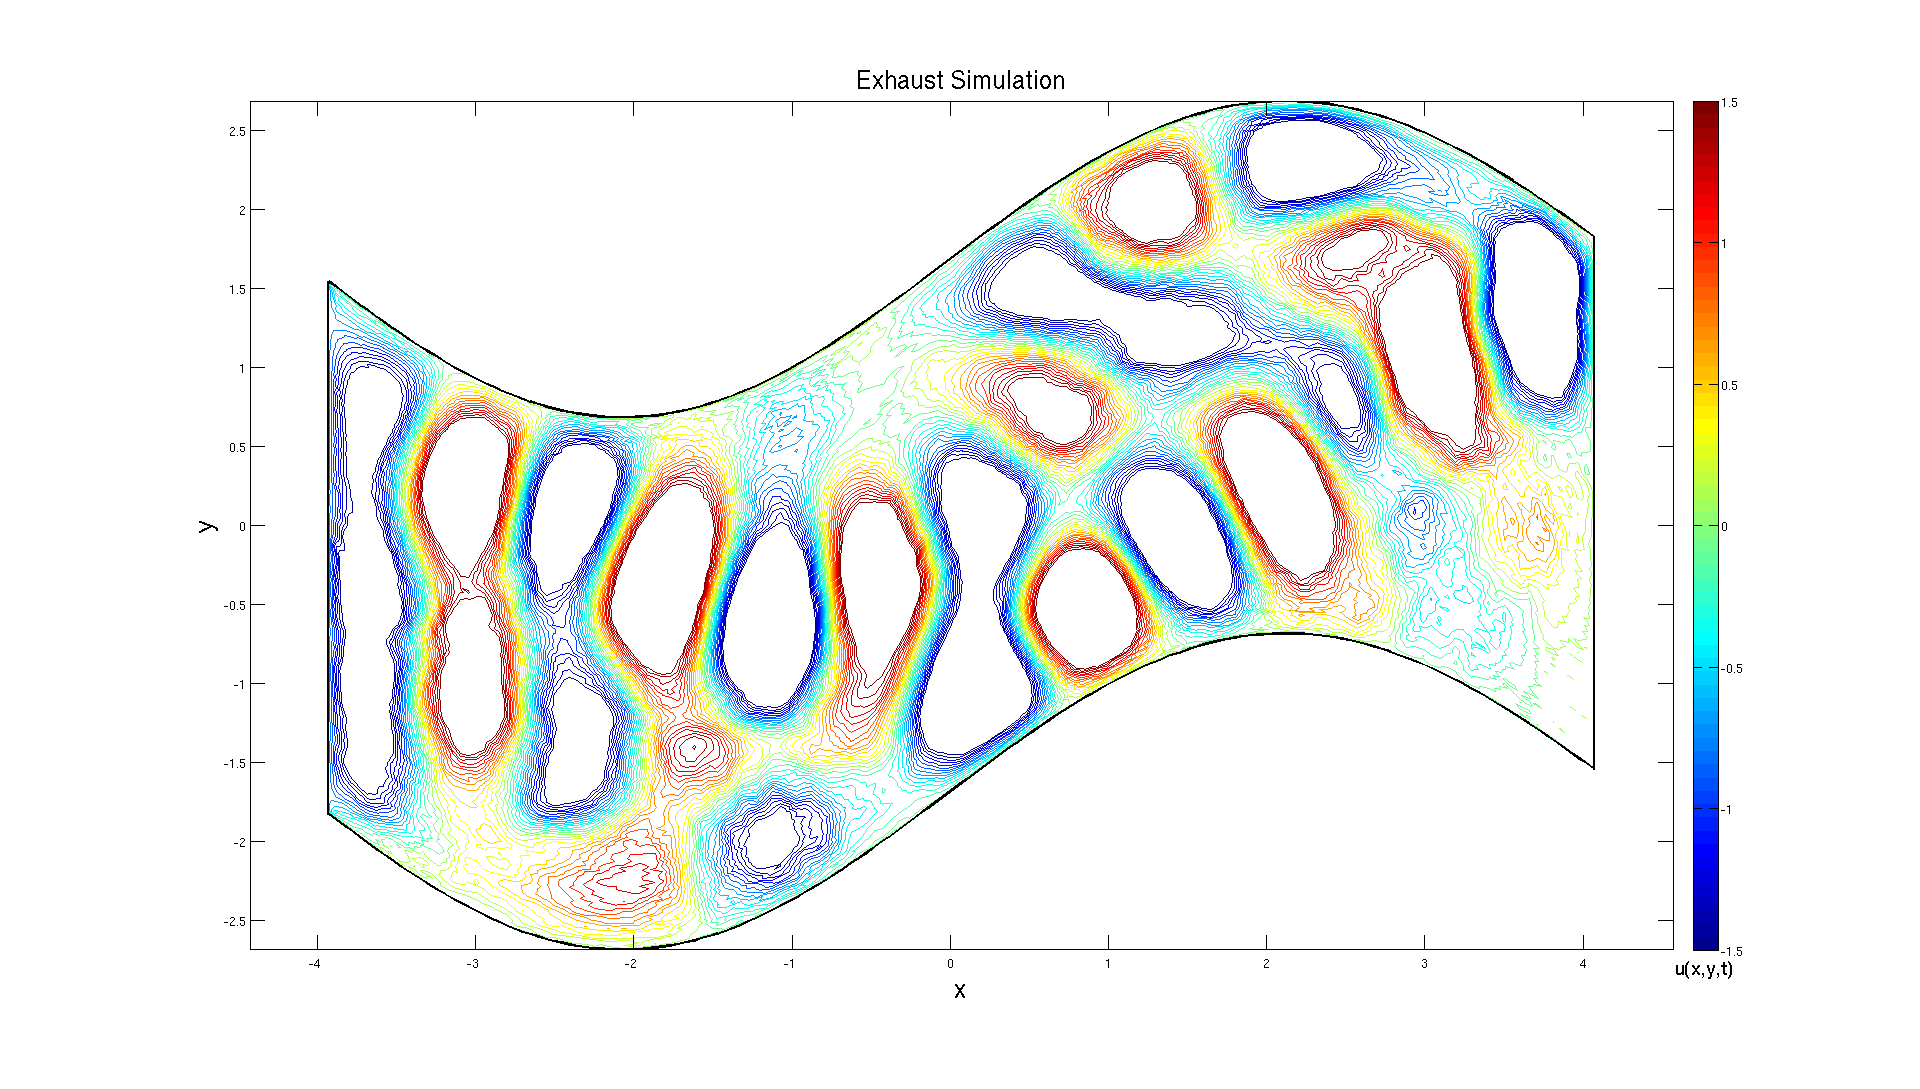
\includegraphics[width=1.0\textwidth]{exhaust_sim_10}
\end{figure}
 

%----------------------------------------------------------------------------------------
%	SECTION 6
%----------------------------------------------------------------------------------------

\section{Strong vs. Weak Scaling (Parallelization)}

Before presenting results, it should be noted what strong and weak scaling are, and why they are different. For strong scaling, the size of the domain is fixed as the number of processors on the domain increase whereas for weak scaling, the size of the domain grows proportional to the number of processors as this number gets larger. The purpose of growing the domain proportional to the number of processors is to fix the domain size inside any of the processors. 
\\
For strong scaling we expect that as the number of processors increases, the cost of communication will also increase and thus will incur more overhead as a result. Then we expect that as P (number of processors) increases, the time it takes for the program to complete will approach a constant value. For weak scaling, since the domain is a fixed size inside each node for any number of processors, then the time it takes for the program to run to completion should remain constant. So then it is expected that weak scaling will be linear.

\begin{table}[h!]
  \centering
  \caption{Experimental results for Strong Scaling}
  \label{tab:table1}
  \begin{tabular}{ccc}
    \toprule
    Some & actual & content\\
    \midrule
    n = 4 & D = 100x100 & time = 0.594162\\
    n = 9 & D = 100x100 & time = 0.358611\\
    n = 16 & D = 100x100 & time = 0.287129\\
    n = 25 & D = 100x100 & time = 0.222724\\
    n = 36 & D = 100x100 & time = 0.210599\\
    \bottomrule
  \end{tabular}
\end{table}
\begin{table}[h!]
  \centering
  \caption{Experimental results for Weak Scaling}
  \label{tab:table1}
  \begin{tabular}{ccc}
    \toprule
    Some & actual & content\\
    \midrule
    n = 4 & D = 20x20 & time = 0.047831\\
    n = 9 & D = 30x30 & time = 0.105451\\
    n = 16 & D = 40x40 & time = 0.145203\\
    n = 25 & D = 50x50 & time = 0.135175\\
    n = 36 & D = 60x60 & time = 0.145983\\
    \bottomrule
  \end{tabular}
\end{table}
\begin{figure}[h]
\caption{Strong vs. Weak Scaling}
\centering
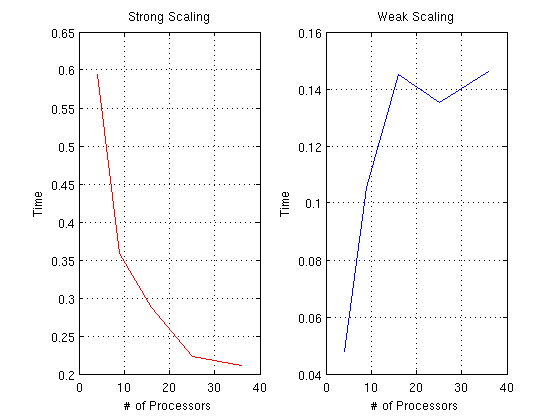
\includegraphics[width=1.0\textwidth]{proc_scaling}
\end{figure}
\newpage
As you can see from the results, our predictions held true for both strong and weak scaling. For strong scaling, it is clear that increasing the number of processors becomes less and less effective, and for weak scaling, the time it takes to complete just about remains constant, which fits the definition of linear scaling for a weak scaling program.



%----------------------------------------------------------------------------------------
%	BIBLIOGRAPHY
%----------------------------------------------------------------------------------------

\newpage
\section{Appendix}
\indent In order to compile and execute the code for this assignment a make file is used:
\\
\begin{center}
\textit{~/Homework/Homework7/Code/}
\end{center}
\\
Once in this directory the following command will compile and execute the code:
\\
\begin{center}
\textit{\$ make \&\& ./homework7.x}
\end{center}
\\
Included in the same directory is a sample simulation video named \(exhaustsim.avi\)
\textbf{MUST WATCH!}
\newpage
\begin{thebibliography}{9}
\bibitem{hw} 
Daniel Appelo
\textit{Homework 7}. 
referenced Dec. 10, 2015

\end{thebibliography}

%----------------------------------------------------------------------------------------


\end{document}